\documentclass[tikz]{standalone}

\usepackage[greek,english]{babel}

\usepackage{pgfplots}
\usetikzlibrary{decorations.pathreplacing}

\pagecolor{white}

\begin{document}
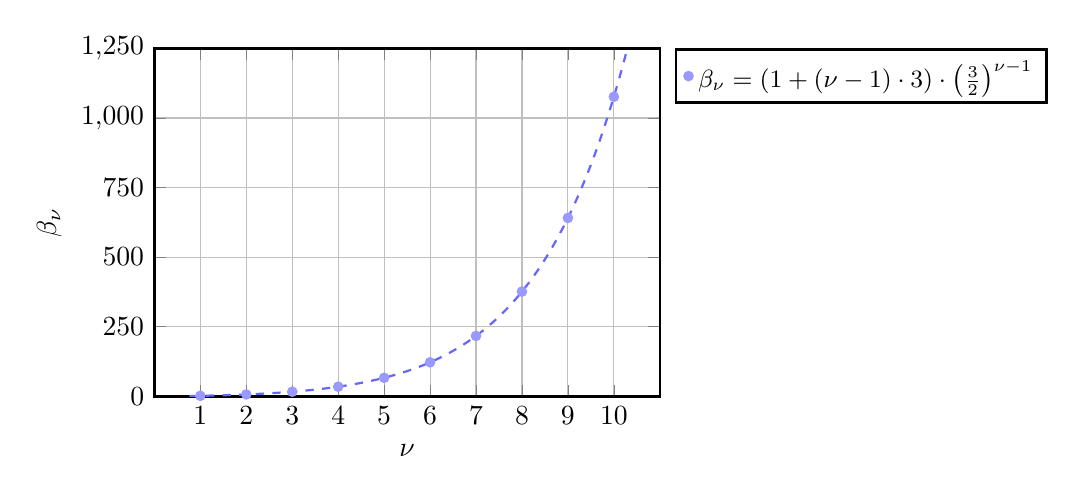
\begin{tikzpicture}
\begin{axis}[
    width=8cm,
    height=6cm,
    domain=-15:15, 
    xmin=0,
    xmax=11,
    ymin=-1.1,
    ymax=1250,
    thick,
    ytick={0,250,500,750,1000,1250},
    xtick=data,
    legend pos=outer north east,
    mark size=1.5pt,
    xlabel={$\nu$},
    ylabel={$\beta_\nu$},
    legend cell align={left},
    grid]


\addplot[only marks, blue!40!white] coordinates {
(1, 1)
(2, 6)
(3, 15.75)
(4, 33.75)
(5, 65.8125)
(6, 121.5)
(7, 216.422)
(8, 375.891)
(9, 640.723)
(10, 1076.41)
};
\addlegendentry{\small $\beta_\nu = (1 + (\nu  -1) \cdot 3) \cdot \left( \frac{3}{2} \right)^{\nu-1}$ }

\addplot[red, domain=0.1:11,restrict y to domain=0:1800, samples=100, blue!60!white,forget plot,dashed]  {(1 + (x-1) * 3) * 1.5^(x-1)};


\end{axis}
\end{tikzpicture}
\end{document}

